%\documentclass{article}
%\usepackage{caption}
%\usepackage{graphicx}
%\begin{document}


%
%%\documentclass{article}
%\usepackage{caption}
%\usepackage{graphicx}
%\begin{document}

\end{document}

%\documentclass{article}
%\usepackage{caption}
%\usepackage{graphicx}
%\begin{document}

\begin{figure}
\begin{minipage}{0.40\textwidth}
  \centering
  
	\begin{center}
	\begin{tabular}{ |c|c|c| } 
 	\hline
 		Item&\emph{U\textsuperscript{cap}}&Support\\ \hline\hline
 		a &  3.00  & 3.00	\\ \hline
 		c &  1.26  & 3.30	\\ \hline
 		d &  1.08  & 1.20	\\ \hline
 		e &  0.54  & 0.60	\\ \hline
 		b &  0.69  & 1.00	\\ \hline
\end{tabular}
\end{center}   
  \captionof{table}{Header Table of US-tree}
\end{minipage}
\hfill
\begin{minipage}{0.40\textwidth}
  \centering
  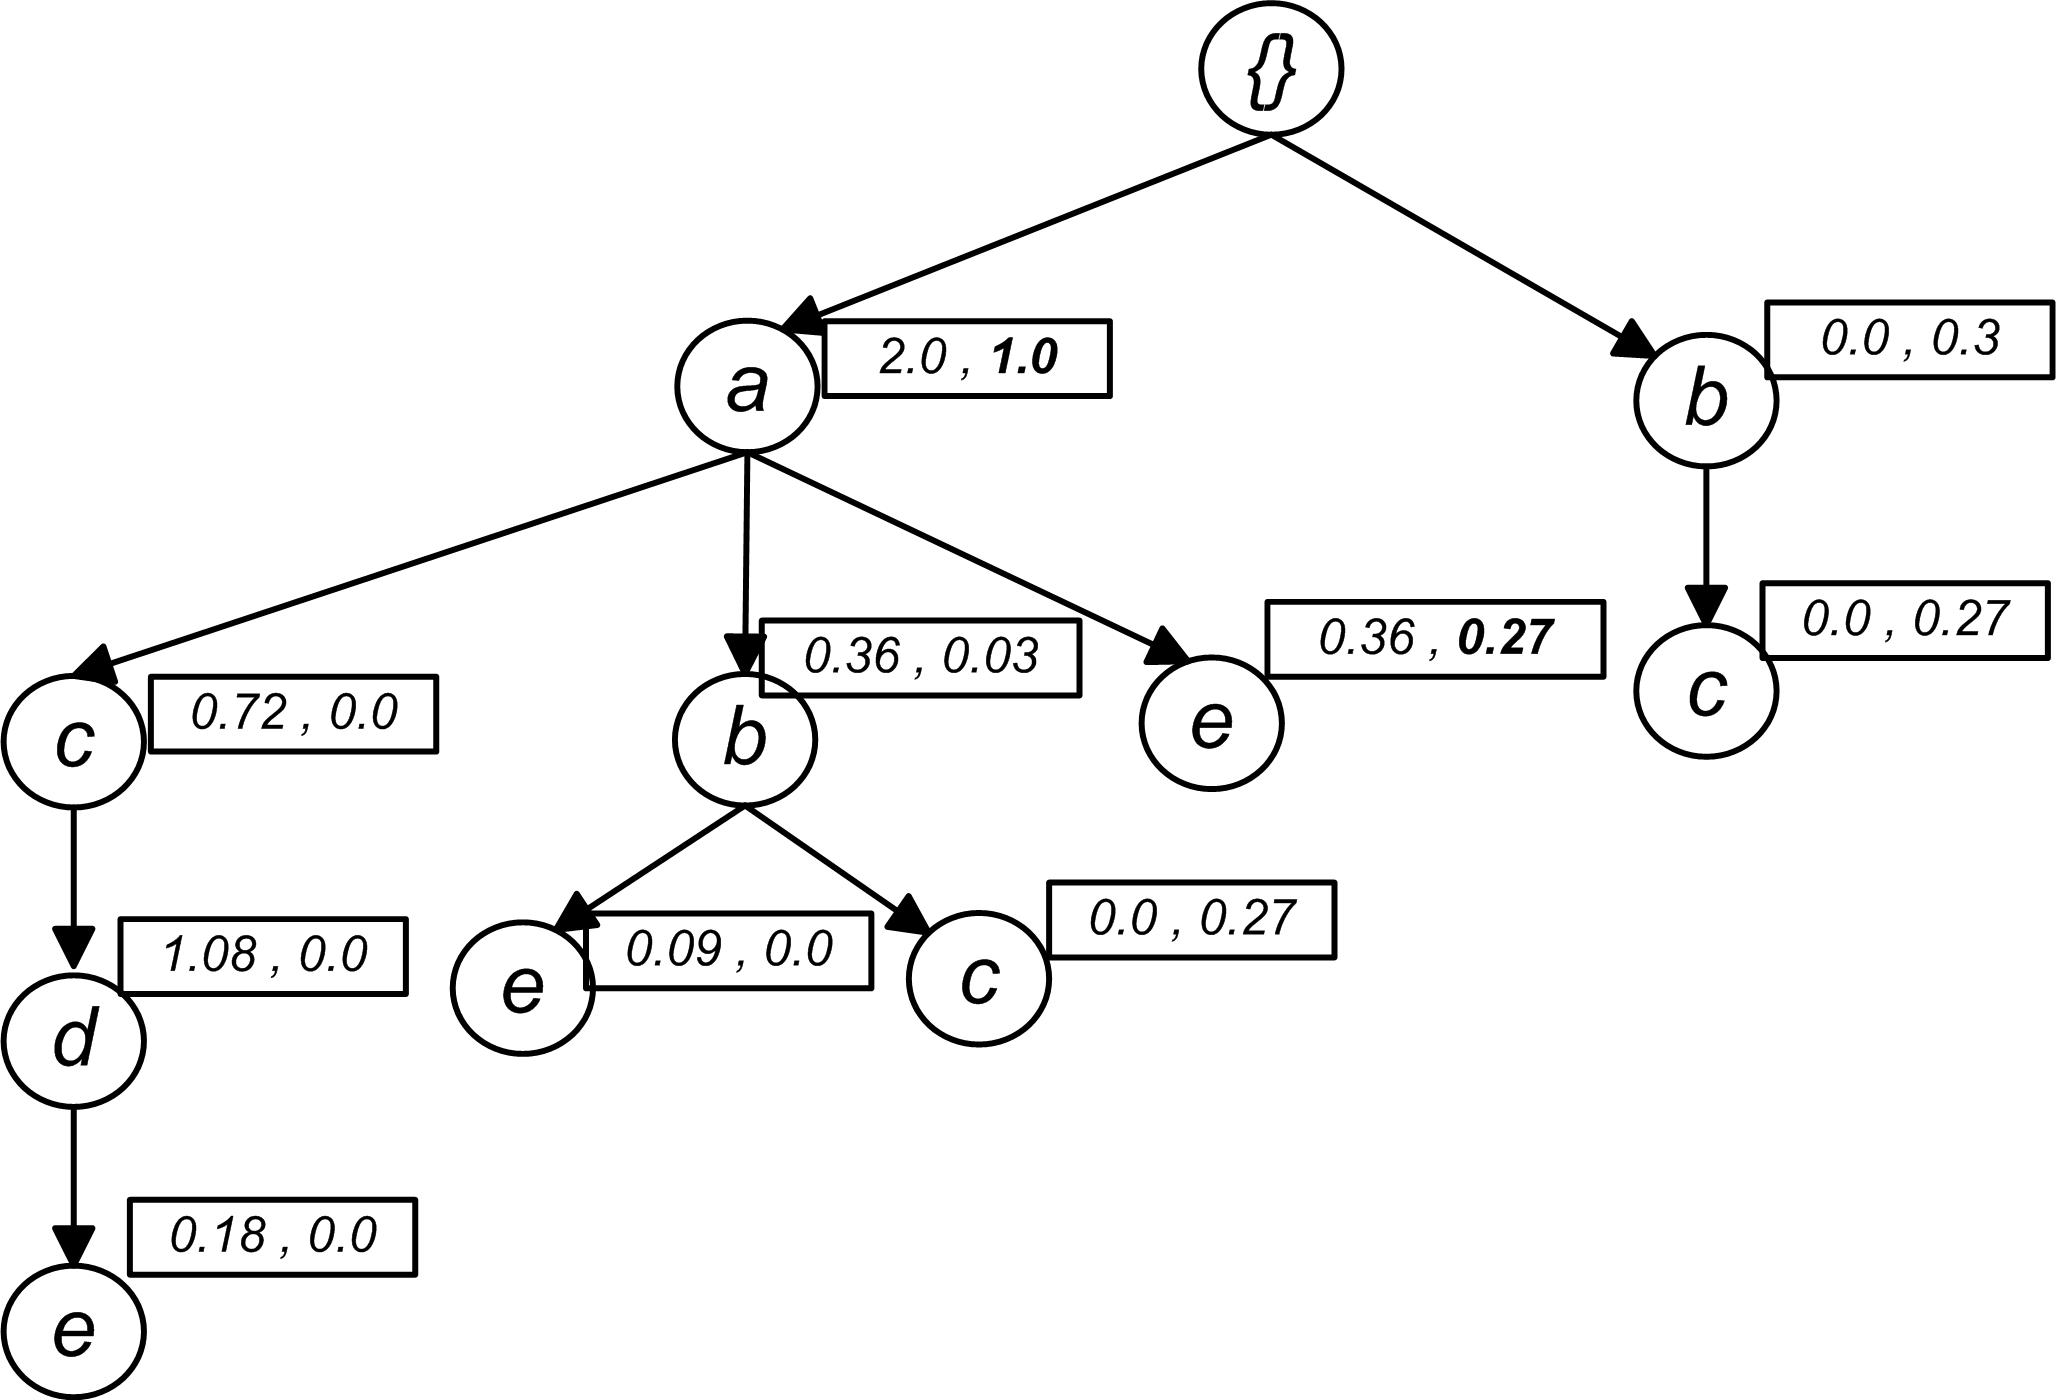
\includegraphics[width=\textwidth]{images/us_tree.jpg}
  \captionof{figure}{US-tree}
\end{minipage}
\caption{US-tree and Header Table}
\label{figure:min_before}
\end{figure}


\begin{figure}
\begin{minipage}{0.40\textwidth}
  \centering
  
	\begin{center}
	\begin{tabular}{ |c|c|c| } 
 	\hline
 		Item&\emph{U\textsuperscript{cap}}&Support\\ \hline\hline
 		a &  3.00  & 3.00\\ \hline
 		c &  1.26  & 3.30\\ \hline
 		d &  1.08  & 1.20\\ \hline
 		b &  0.69  & 1.00\\ \hline
\end{tabular}
\end{center}  
  
  
  \captionof{table}{Header Table for Mining}
\end{minipage}
\hfill
\begin{minipage}{0.40\textwidth}
  \centering
  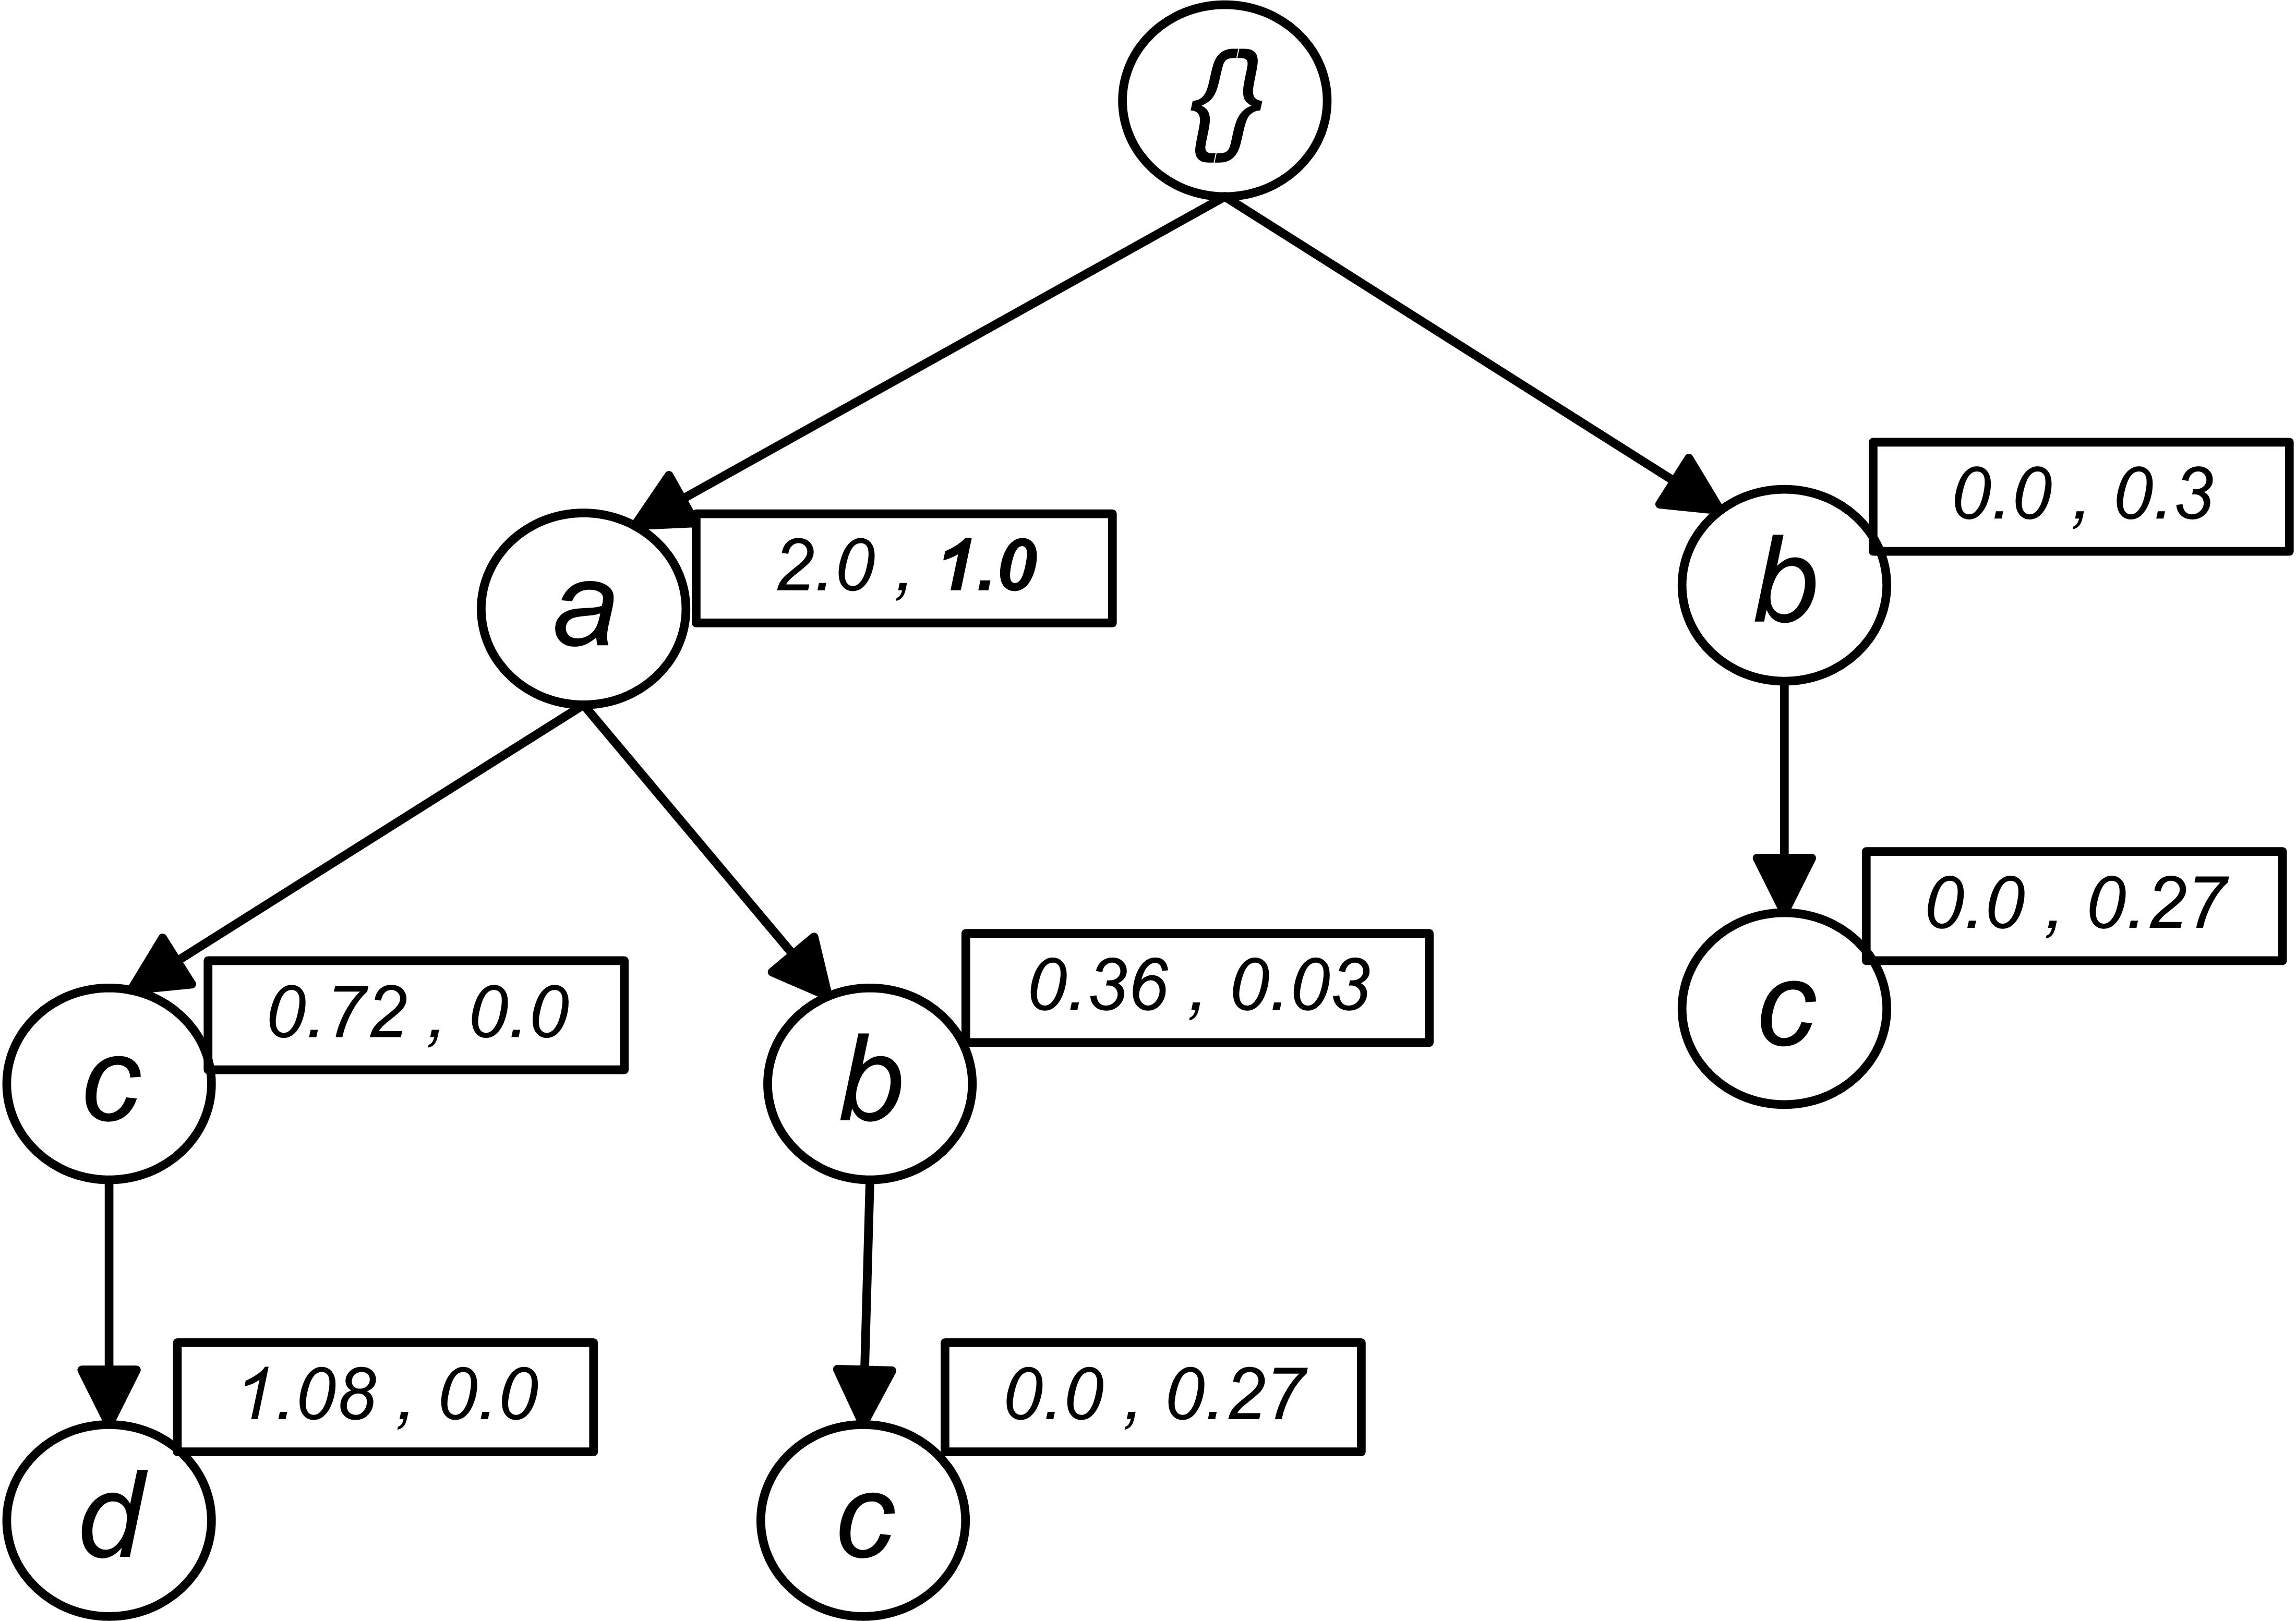
\includegraphics[width=\textwidth]{images/M_TREE.jpg}
  \captionof{figure}{US-tree for Mining}
\end{minipage}
\caption{US-tree and Header Table for Mining}
\label{figure:min_ready}
\end{figure}
%\end{document}
\paragraph{}
In this section we will discuss about our proposed approach for mining frequent pattern over large uncertain stream data. Stream Data has a special property that it comes and flows away. For this reason we will lose data after data stream has flown away. To resolve this we will proposed a window based approach where we will keep the most recent information in a tree structure as the most recent data is most valuable. Later we will show how the window will slide, remove old data and insert new data in the window. As, for uncertain data stream each same item in different transaction has different existential probability, it becomes very hard to merge (share) this node in the tree. This uncertainty property of item makes the tree huge. We have proposed a new \emph{U\textsuperscript{cap}} value for each item that helps to share a single node when constructing the tree which we named as \emph{US-tree}. We will show that our proposed tree \emph{US-tree} will be very compact and very efficient for later mining. Later will describe an approach for mining the \emph {US-tree} named \emph{USFP-growth} which is \emph{FP-growth} like approach. Later we will propose a method for filtering false positive from found most probable frequent patterns.\\ \\ \\

%\documentclass{article}
%\usepackage{caption}
%\usepackage{graphicx}
%\begin{document}
\begin{figure}
\begin{minipage}{0.40\textwidth}
  \centering
	\begin{center}
	\begin{tabular}{ |c|c| } 
 	\hline
 		Item&Value\\ \hline\hline
 		a &  1.08  	\\ \hline
 		c &  1.08   	\\ \hline
 		
\end{tabular}
\end{center}  
  \captionof{table}{\emph{d-cond tree} Header }
\end{minipage}
  \hfill
\hfill
\begin{minipage}{0.23\textwidth}
  \centering
  \hfill
  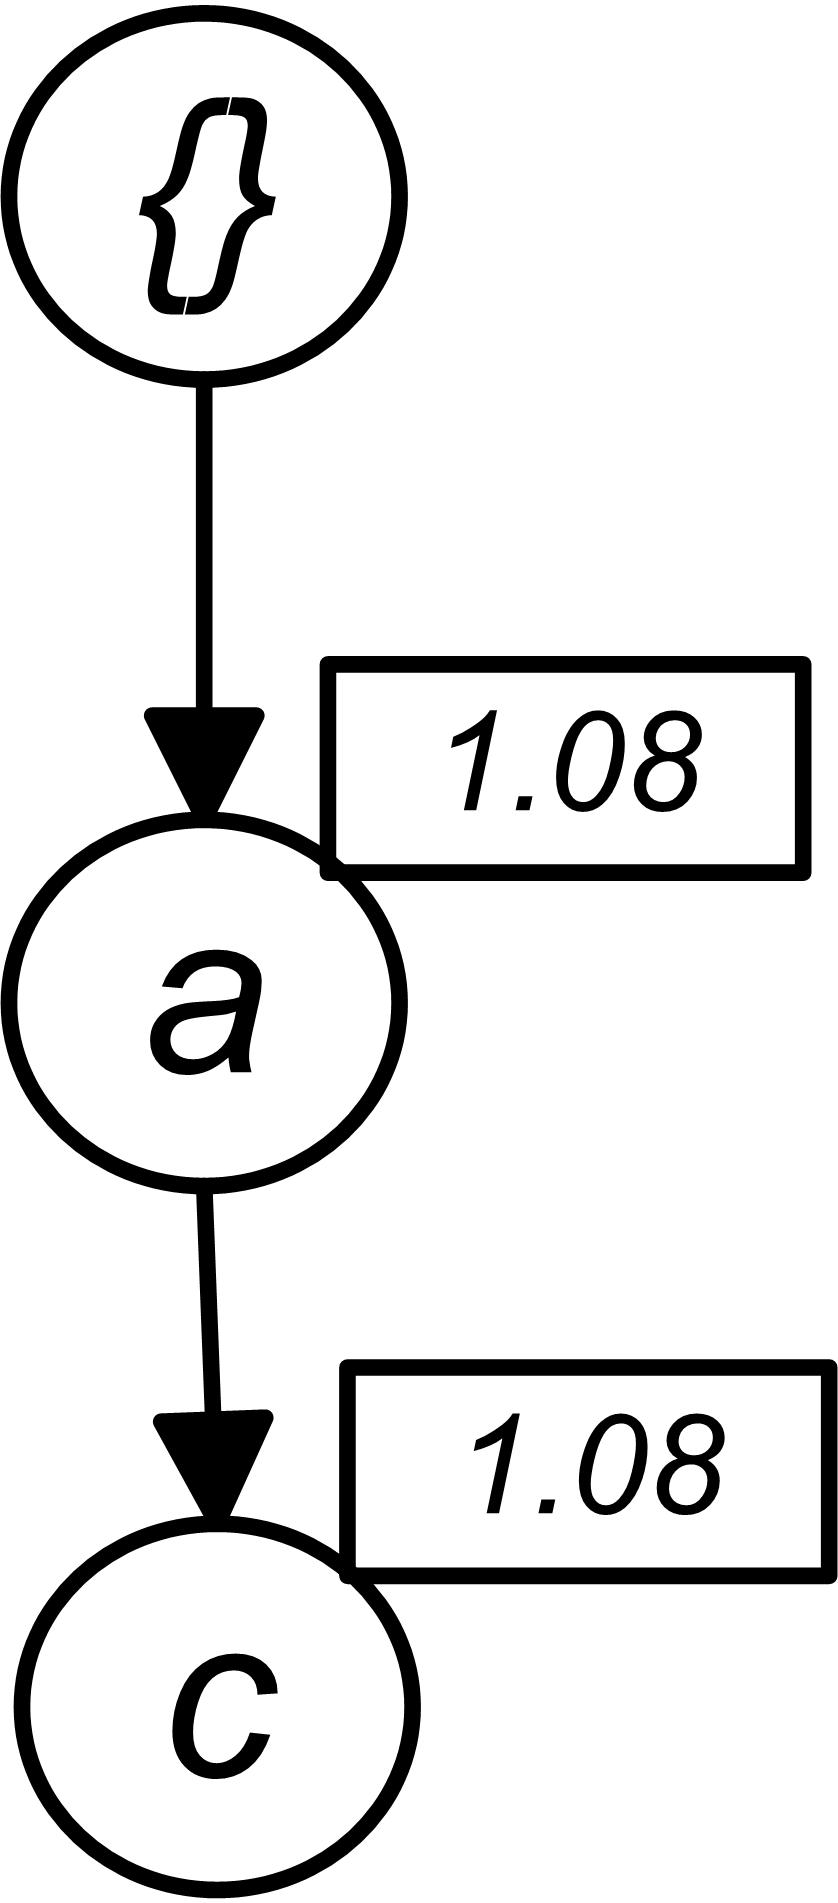
\includegraphics[width=.8\textwidth, height=5cm]{images/D_COND.jpg}
  \hfill
\end{minipage}
\hfill
\begin{minipage}{0.30\textwidth}
  \centering
  
	\begin{center}
	\begin{tabular}{ |c| } 
 	\hline
 		Freq Patterns \\ \hline\hline
 		dc  	\\ \hline
 		da   	\\ \hline
 		dca   	\\ \hline
 		
\end{tabular}
\end{center}  
  \captionof{table}{ \emph{Frequent Patterns} }
\end{minipage}
\caption{\emph{d-cond} Tree and corresponding Header}
\label{figure:d_cond}
\end{figure}
\begin{figure}
\begin{minipage}{0.30\textwidth}
  \centering
	\begin{center}
	\begin{tabular}{ |c|c| } 
 	\hline
 		Item&Value\\ \hline\hline
 		a &  .99  	\\ \hline
 		b &  .54   	\\ \hline
\end{tabular}
\end{center}  
  \captionof{table}{Header }
\end{minipage}
  \hfill
\begin{minipage}{0.29\textwidth}
  \centering
  \hfill
  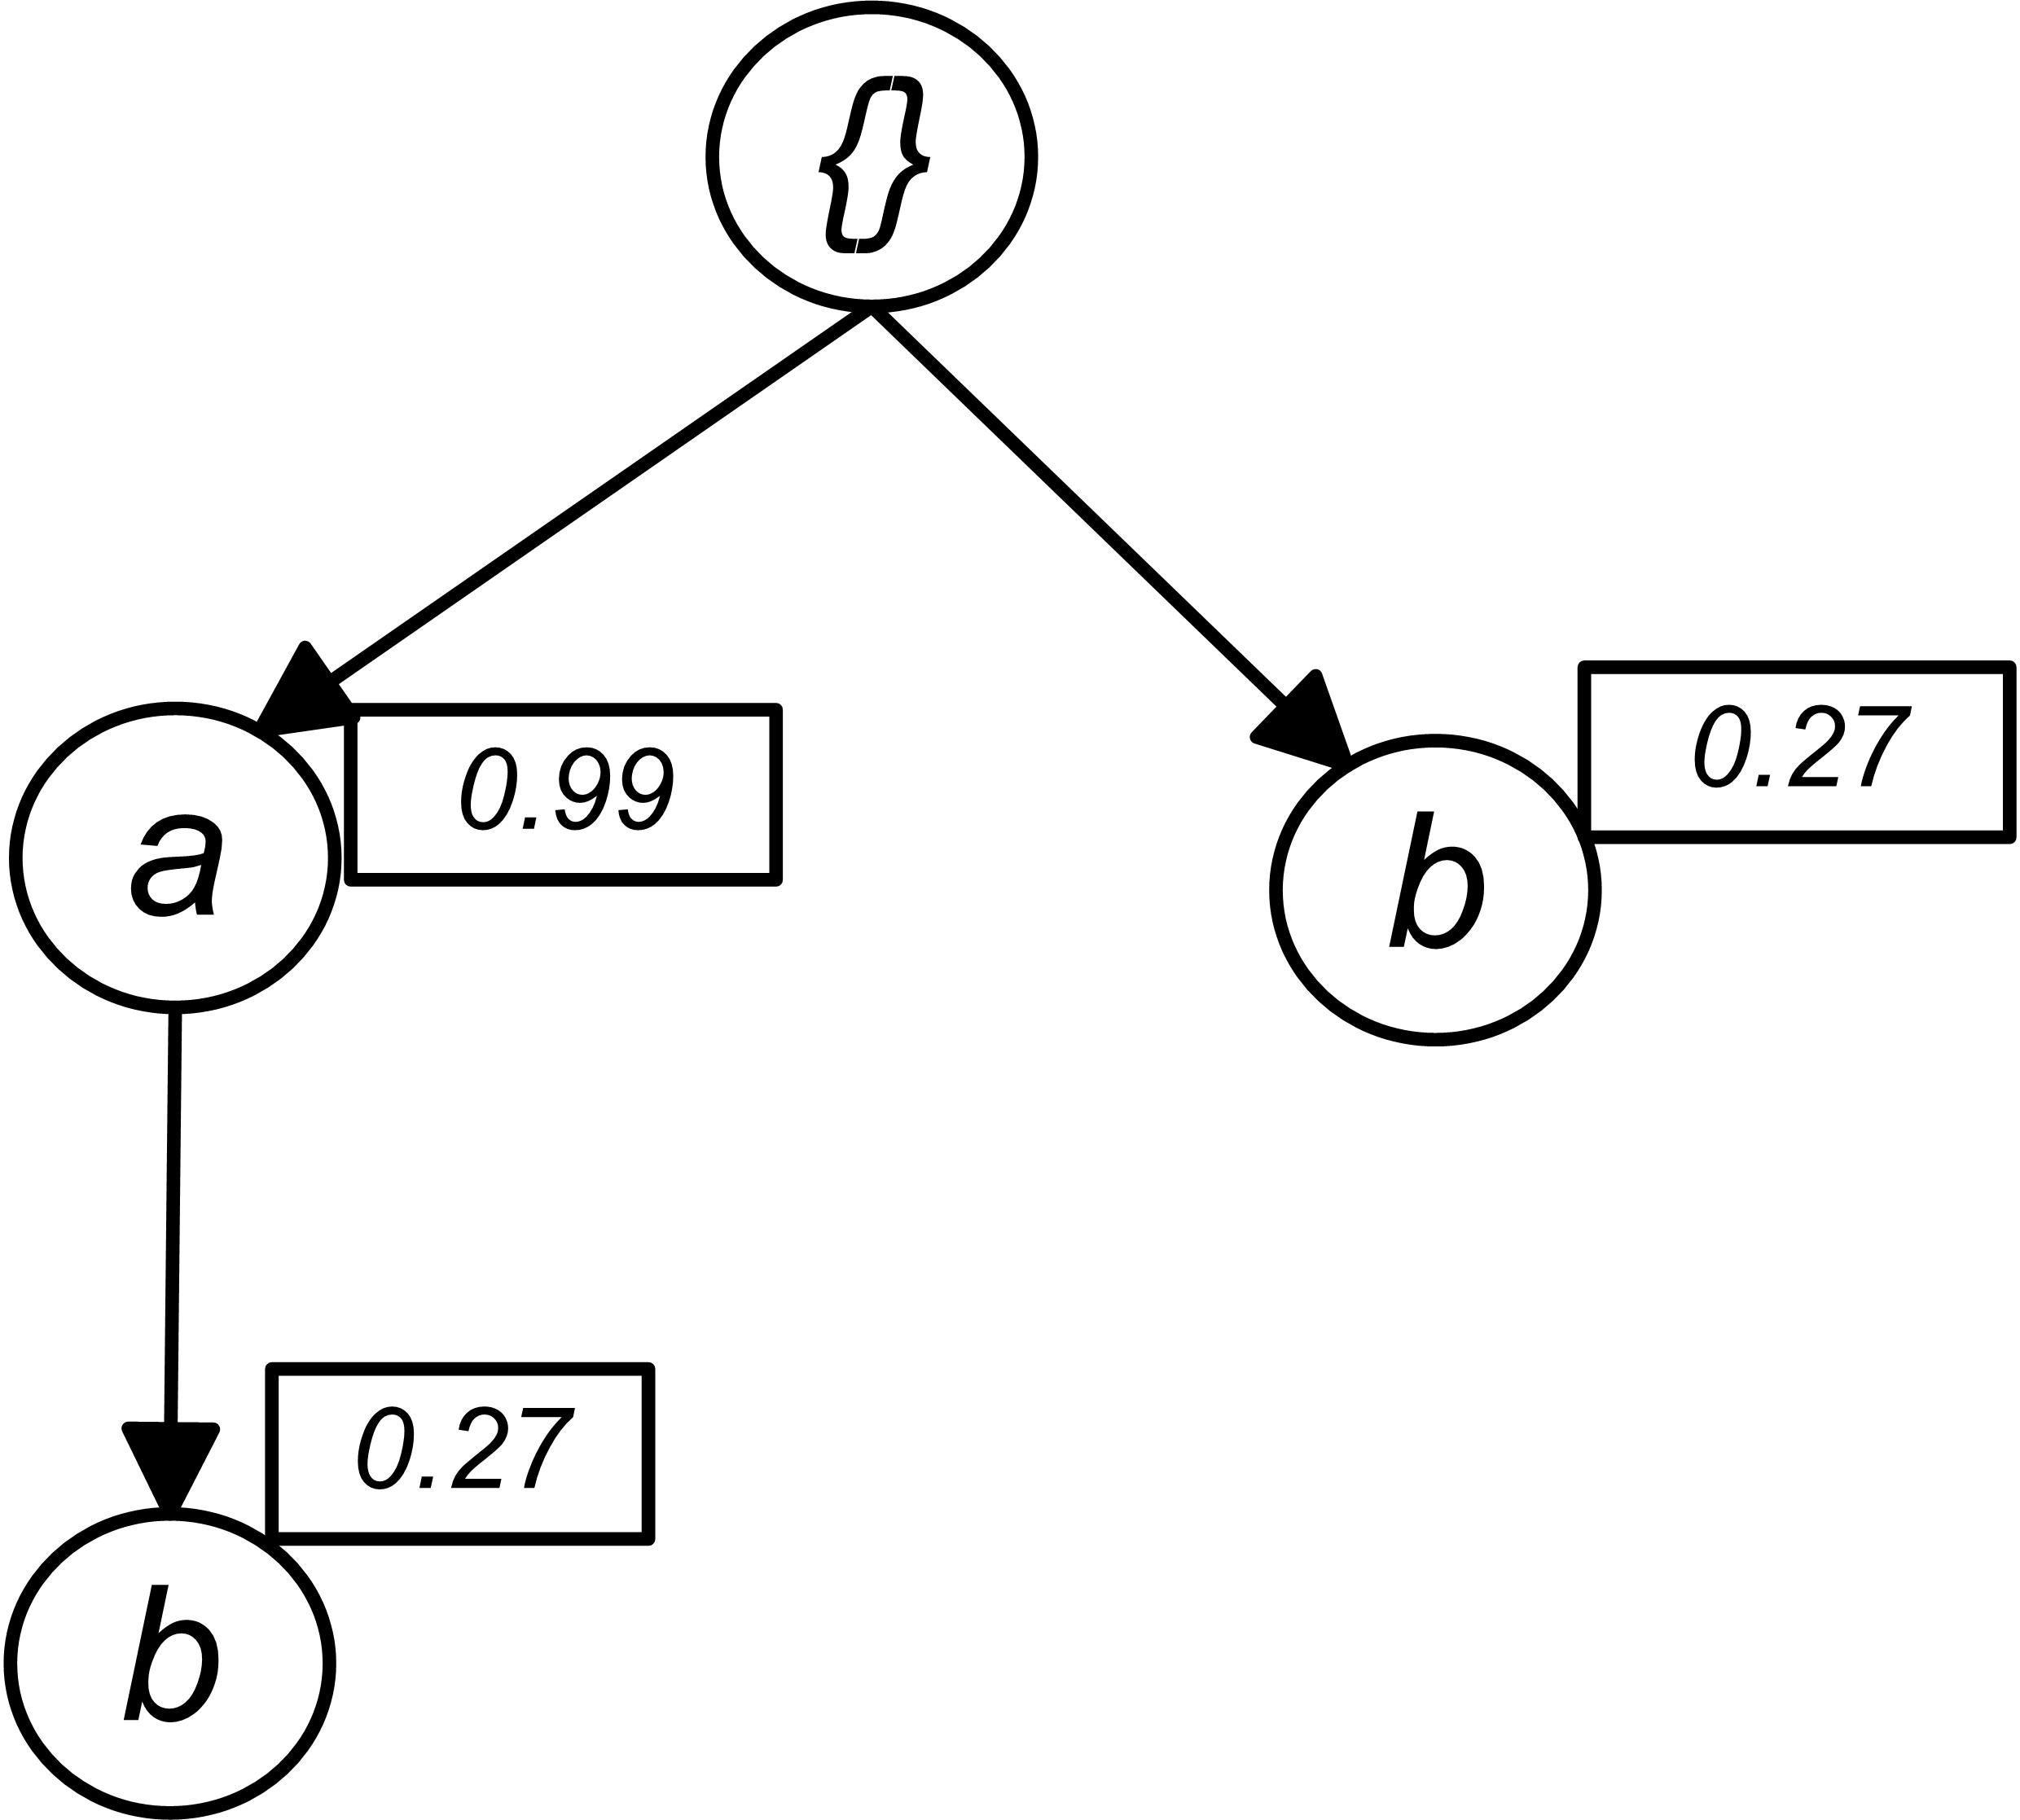
\includegraphics[width=.8\textwidth, height=3.5cm]{images/C_COND.jpg}
  \hfill  
\end{minipage}
\hfill
\begin{minipage}{0.30\textwidth}
  \centering  
	\begin{center}
	\begin{tabular}{ |c| } 
 	\hline
 		Freq Patterns \\ \hline\hline
 		ca  	\\ \hline
 		
\end{tabular}
\end{center}   
  \captionof{table}{ \emph{Freq Patterns} }
\end{minipage}
\caption{\emph{c-cond} Tree and corresponding Header}
\label{figure:c_cond}
\end{figure}
\begin{figure}
\centering
  
\includegraphics[width=.10\textwidth, height=1.1cm]{images/A_COND.jpg}
\caption{\emph{a-cond} Tree}
\label{figure:a_cond}
\end{figure}

%\end{document}


%
%\end{document}